\documentclass[12pt, a4paper]{article}
\usepackage[utf8]{inputenc}
\usepackage{amsmath}
\usepackage{amsfonts}
\usepackage{amssymb}
\usepackage{graphicx} % Required for inserting images
\usepackage[left=2.5cm, right=2.5cm, top=2.5cm, bottom=2.5cm]{geometry}
\usepackage{hyperref} % For clickable links
\usepackage{color} % For coloring text
\usepackage{listings} % For code snippets

% The TikZ packages are commented out as they are not needed for image inclusion
% and were causing compilation issues.
% \usepackage{tikz} % For drawing diagrams
% \usetikzlibrary{graphs, graphdrawing, arrows.meta, positioning}
% \usegdlibrary{trees} % For hierarchical diagrams

% Define custom colors
\definecolor{codegreen}{rgb}{0,0.6,0}
\definecolor{codegray}{rgb}{0.5,0.5,0.5}
\definecolor{codepurple}{rgb}{0.58,0,0.82}
\definecolor{backcolour}{rgb}{0.98,0.98,0.98}

% Listing style for code snippets
\lstdefinestyle{mystyle}{
    backgroundcolor=\color{backcolour},
    commentstyle=\color{codegreen},
    keywordstyle=\color{magenta},
    numberstyle=\tiny\color{codegray},
    stringstyle=\color{codepurple},
    basicstyle=\ttfamily\footnotesize,
    breakatwhitespace=false,
    breaklines=true,
    captionpos=b,
    keepspaces=true,
    numbers=left,
    numbersep=5pt,
    showspaces=false,
    showstringspaces=false,
    showtabs=false,
    tabsize=2
}
\lstset{style=mystyle}

\title{A Framework for Natural Language DSL Interaction}
\author{System Documentation}
\date{\today}

\begin{document}

\maketitle
\tableofcontents
\newpage

\section{Introduction}
This document outlines the architecture of a reusable framework designed to create natural language interfaces for Domain Specific Languages (DSLs). The system uses a Large Language Model (LLM) to parse user intent from text. This intent is then translated into a formal DSL command for execution.

The framework is designed to be domain-agnostic. A new domain can be integrated by providing a set of configuration files that define the domain's language and capabilities. This document uses an "Event Management" DSL as a concrete implementation example to illustrate the framework's components.

\section{Overall System Architecture}
The framework is divided into several logical layers. This modular design separates concerns and allows for extensibility. The high-level interaction flow is depicted in Figure \ref{fig:overall_architecture}.

\begin{figure}[h!]
    \centering
    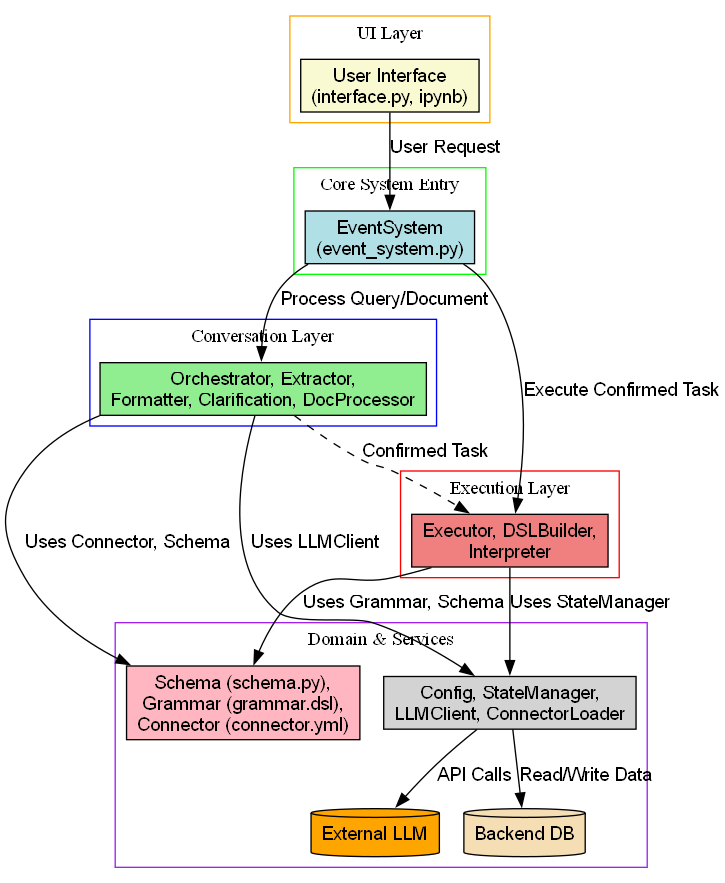
\includegraphics[width=0.9\textwidth]{overall_architecture.png}
    \caption{Overall System Architecture Diagram}
    \label{fig:overall_architecture}
\end{figure}

\subsection{Architectural Layers}

\subsubsection{1. User Interface (UI) Layer}
\textbf{Core Components:} \texttt{interface.py}, Notebook file

This layer is the client-facing component. It handles the rendering of the conversational interface and captures all user input. It is a client of the core system coordinator.

\textbf{Key Responsibilities:}
\begin{itemize}
    \item Displaying conversation history.
    \item Capturing user queries from an input field.
    \item Rendering system responses, including formatted summaries and clarification requests.
    \item Managing UI state, such as waiting for a user confirmation.
\end{itemize}

\subsubsection{2. Core System Entry Point}
\textbf{Core Component:} \texttt{event\_system.py} (example name)

This class acts as the central coordinator. It instantiates and holds references to the primary sub-systems (Orchestrator, Executor, etc.) and delegates incoming requests from the UI to the appropriate components.

\textbf{Key Responsibilities:}
\begin{itemize}
    \item Receiving user queries from the UI.
    \item Routing requests to the Conversation or Execution layers.
    \item Providing a unified interface to the underlying system functionalities.
\end{itemize}

\subsubsection{3. Conversation Layer}
\textbf{Core Components:} \texttt{orchestrator.py}, \texttt{extractor.py}, \texttt{formatter.py}, \texttt{clarification.py}

This layer contains the logic for managing the natural language dialogue. Its primary function is to transform unstructured user text into a structured, validated command that can be passed to the Execution Layer.

\textbf{Key Responsibilities:}
\begin{itemize}
    \item \textbf{Orchestration (\texttt{orchestrator.py}):} Manages the conversation state and flow. It coordinates the extractor, validator, and formatter to process a user request.
    \item \textbf{Extraction (\texttt{extractor.py}):} Uses an LLM to parse a user query into a structured object containing an \texttt{action} and its associated \texttt{parameters}. This process is guided by the domain's \texttt{connector.yml} file.
    \item \textbf{Formatting (\texttt{formatter.py}):} Generates user-facing messages, such as the "Here is what I understood" summary.
    \item \textbf{Clarification (\texttt{clarification.py}):} Identifies missing required parameters and generates prompts to ask the user for the necessary information.
\end{itemize}

\begin{figure}[h!]
    \centering
    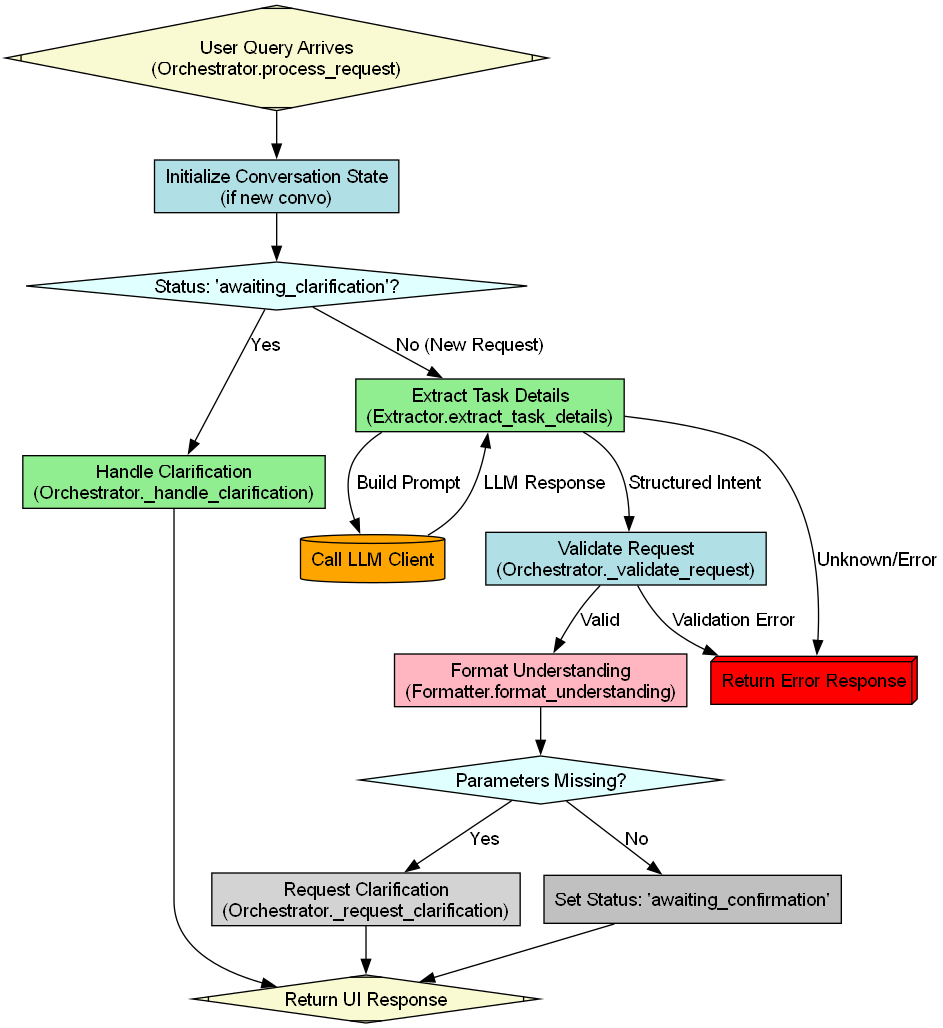
\includegraphics[width=0.9\textwidth]{conversation_flow.png}
    \caption{Conversation Flow within the Orchestrator}
    \label{fig:conversation_flow}
\end{figure}


\subsubsection{4. Execution Layer}
\textbf{Core Components:} \texttt{executor.py}, \texttt{dsl\_builder.py}, \texttt{interpreter.py}

After a command has been fully specified and confirmed by the user, the Execution Layer is responsible for its formal execution.

\textbf{Key Responsibilities:}
\begin{itemize}
    \item \textbf{Execution (\texttt{executor.py}):} Manages the execution process by invoking the DSL builder and the interpreter.
    \item \textbf{DSL Building (\texttt{dsl\_builder.py}):} Converts the structured command object (action and parameters) into a formal DSL string that conforms to the domain's grammar.
    \item \textbf{Interpretation (\texttt{interpreter.py}):} A domain-specific component that parses the DSL string and executes the logic associated with the command, modifying the application state.
\end{itemize}

\begin{figure}[h!]
    \centering
    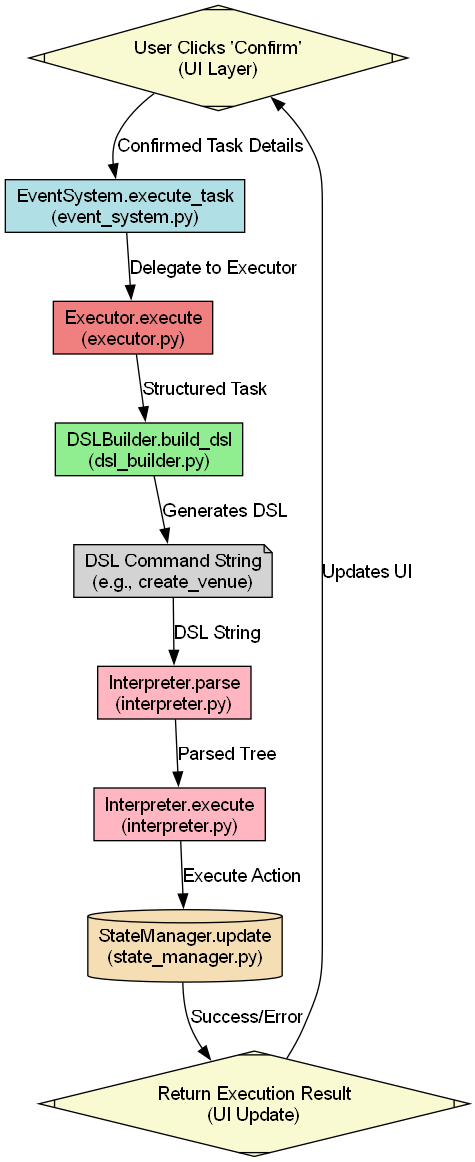
\includegraphics[width=0.9\textwidth]{execution_flow.png}
    \caption{Execution Flow Diagram}
    \label{fig:execution_flow}
\end{figure}

\subsubsection{5. Core Services}
\textbf{Core Components:} \texttt{config.py}, \texttt{state\_manager.py}, \texttt{llm\_client.py}, \texttt{connector\_loader.py}

These components provide foundational utilities used across the framework.

\textbf{Key Responsibilities:}
\begin{itemize}
    \item \textbf{Configuration (\texttt{config.py}):} Centralizes application settings.
    \item \textbf{State Management (\texttt{state\_manager.py}):} Provides an interface for persistent storage (e.g., to a JSON file).
    \item \textbf{LLM Client (\texttt{llm\_client.py}):} Abstracts the communication logic for different LLM APIs.
    \item \textbf{Connector Loader (\texttt{connector\_loader.py}):} Loads and caches the domain's \texttt{connector.yml} file.
\end{itemize}

\subsubsection{6. Domain Definition}
\textbf{Core Components:} \texttt{schema.py}, \texttt{grammar.dsl}, \texttt{connector.yml}

To integrate a new DSL, a developer must provide these three domain-specific configuration files.

\textbf{Key Responsibilities:}
\begin{itemize}
    \item \textbf{Schema (\texttt{schema.py}):} A Python dictionary that formally defines the domain's actions, their required and optional parameters, and associated role-based permissions.
    \item \textbf{DSL Grammar (\texttt{grammar.dsl}):} A Lark grammar file that defines the formal syntax of the DSL for the interpreter.
    \item \textbf{Connector (\texttt{connector.yml}):} A YAML file that provides natural language descriptions and prompts for all actions and parameters. This file is used to construct the prompts for the LLM.
\end{itemize}

\section{Conclusion}
This framework provides a layered architecture for translating natural language into executable DSL commands. By separating the concerns of conversation management, execution, and domain definition, the system is extensible to new domains. A developer can define a new natural language interface by supplying the three domain-specific files: a schema, a grammar, and a connector.

\end{document}